% 论文关系类数据图内嵌效果演示（relationship.md 指导）
% 编译：xelatex -interaction=nonstopmode paper_embedded_relationship.tex（两遍，交叉引用）
\documentclass[12pt]{ctexart}
\ctexset{fontset=none}
\usepackage[a4paper, margin=2.6cm]{geometry}
\usepackage{graphicx}
\usepackage{caption}
\captionsetup{font=small, labelsep=quad}
\setcounter{section}{2}
\renewcommand{\thefigure}{\thesection.\arabic{figure}}
% ============================================================
% pretty-charts 字体层：衬线搭配（宋体 + Times New Roman）
% 用法：\input{.../references/style/tikz/fonts-serif.tex}
%
% 为什么单独成文件：示例此前各自写 \setmainfont{Times New Roman}
% + \setCJKmainfont{SimSun}，这两个字体只存在于 Windows，同一份示例在
% Linux/macOS 上无法编译（CI 也就无从编译）。这里按"字体是否存在"逐级回退：
%   Windows  → Times New Roman + SimSun（与原行为完全一致）
%   Linux    → TeX Gyre Termes + Noto Serif CJK SC（apt install fonts-noto-cjk-extra）
%   兜底     → TeX Gyre Termes + FandolSong（TeX Live 自带）
%   再兜底   → 只发警告、不设字体，保证编译不因缺字体而失败（中文可能显示异常）
% \IfFontExistsTF 由 fontspec 提供（preamble.tex 已加载 fontspec）。
% ============================================================
\IfFontExistsTF{Times New Roman}
  {\setmainfont{Times New Roman}}
  {\setmainfont{TeX Gyre Termes}}          % TeX Live 自带，Times 的开源等价物
\IfFontExistsTF{SimSun}
  {\setCJKmainfont{SimSun}}                % 中文宋体（Windows）
  {\IfFontExistsTF{Noto Serif CJK SC}
     {\setCJKmainfont{Noto Serif CJK SC}}   % Linux（fonts-noto-cjk-extra）
     {\IfFontExistsTF{FandolSong}
        {\setCJKmainfont{FandolSong}}        % 兜底：TeX Live 自带，无需系统字体包
        {\PackageWarning{pretty-charts}{未找到中文衬线字体（已尝试 SimSun / %
          Noto Serif CJK SC / FandolSong）；中文可能显示异常。%
          请安装 fonts-noto-cjk-extra，或改用 fonts-sans.tex}}}}


\begin{document}
\section{系统设计与实现}

营销投入与销售额的关系因渠道而异：线上渠道的边际回报明显高于线下渠道。当样本量
增大时，散点图需要密度化处理以避免过绘；第三维度（公司规模）则以气泡面积编码。
三种表达方式如图~\ref{fig:rel}~所示。

\begin{figure}[htbp]
  \centering
  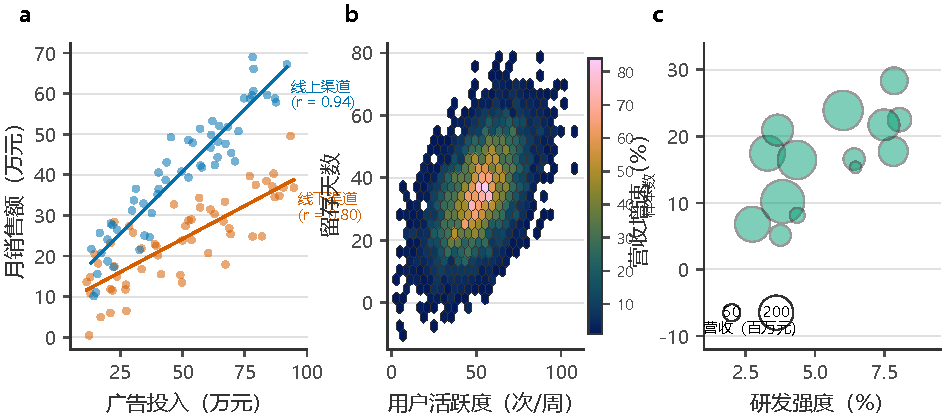
\includegraphics[width=\linewidth]{fig1.pdf}
  \caption{广告投入与月销售额的关系。(a)~分渠道散点及线性回归（阴影为 95\% 置信带，
  拟合范围不外推出数据范围；$n=55$/组）；(b)~全样本（$n=6000$）的六边形二维密度，
  颜色为面板内样本数；(c)~气泡图中气泡面积与公司营收成正比，左下角为参照气泡
  （50 与 200 百万元）。相关仅描述统计关联，不构成因果解释。}
  \label{fig:rel}
\end{figure}

如图~\ref{fig:rel}~(a)~所示，线上渠道的回归斜率（0.58）约为线下渠道（0.32）的
1.8 倍，两渠道 95\% 置信带在广告投入超过 60 万元后完全分离。(b)~采用六边形分箱：
样本量超过 2000 时普通散点必然过绘，密度化后中心高密度区与尾部稀疏区清晰可辨。
(c)~中气泡面积编码营收规模（半径为平方根），并以参照气泡定标，读者无需查图例
即可估计任意气泡的量级。

\end{document}
